\section{队列、停止与续跑}

服务同一时刻只跑一轮。再按执行时任务进队列，按钮变成“\texttt{排队运行}”，当前这轮结束自动开始。排队在内存里，重启服务会清空，
所以别把排队当定时任务。队列里有些任务永远起不来：画布走不通、复用的节点坏掉、模型提供方写错，
这类任务入队时就被标上丢弃，轮到时直接跳过并在控制台说明原因，不会一直挡在队首。

停止按钮把正在跑的与还没跑的节点一起停下。已经写下的行保留，节点标成停止，不算失败；有些节点停在一半时把没处理的行留成未处理，
节点算部分完成。这个区别在写方法段时有用。

所有输出与模型答案都落盘，所以一条长链可以分几次做完。

\begin{figure}[H]\centering
\begin{tikzpicture}[node distance=10mm,scale=0.95,transform shape]
  \node[card=src,text width=2.6cm] (run) {运行中};
  \node[card=anl,right=of run,text width=2.8cm] (stop) {中断\\[1pt]\micro 停止、关服务、断电};
  \node[card=viz,right=of stop,text width=2.8cm] (open) {重新打开画布\\[1pt]\micro 顶部横幅};
  \node[card=okc,below=8mm of open,text width=2.8cm] (cont) {继续\\[1pt]\micro 只补缺失部分};
  \node[chip,below=8mm of stop,text width=2.8cm] (fresh) {重新开始\\[1pt]\micro 全量重跑};
  \draw[wire] (run) -- (stop);
  \draw[wire] (stop) -- (open);
  \draw[wire] (open) -- (cont);
  \draw[softwire] (open) -- (fresh);
  \node[micro,right=2mm of cont,text width=3.0cm,align=left] {模型答案走缓存\\ 已付过的钱不再付};
  \node[micro,right=2mm of fresh,text width=3.0cm,align=left] {链短、结果可疑时\\ 用它干净地重来};
\end{tikzpicture}
\caption{中断以后的两条路}
\label{fig:resume}
\end{figure}

重新打开工作流，顶部出现一条检测到中断的运行的横幅。点“\texttt{继续}”，程序只补缺失的部分：已经完成的节点直接复用，
已经处理过的行不再重跑，模型答案从缓存里取。点“\texttt{重新开始}”才算全量重来。

平台那边已经登出、或者数据已经花过钱采过，可以拖一个“\texttt{断点续跑}”节点，直接把历史运行的输出行收过来当输入，从那里接着往下做。
它不重新爬，只读取已经存下的行。

节点完成以后，只要上游没变，再次运行到它就复用上次的结果，新加几个节点也不影响旧的。要让某个节点重算，用“\texttt{从此节点重跑}”，
它和下游重算，上游照旧拿。

\section{运行台账}

运行记录里有一行一次的运行编号、工作流名、状态、模式、开始与结束时间、节点数、行数。每个节点每次运行的表格输出按运行号存着，
随时能翻出来看真实的行，也能导出。日志按运行号持久化，按级别与工作流过滤，能下载成文本。右侧的动作能载入这次结果到画布、
打开日志、生成报告、删除这条记录。

\begin{figure}[H]\centering
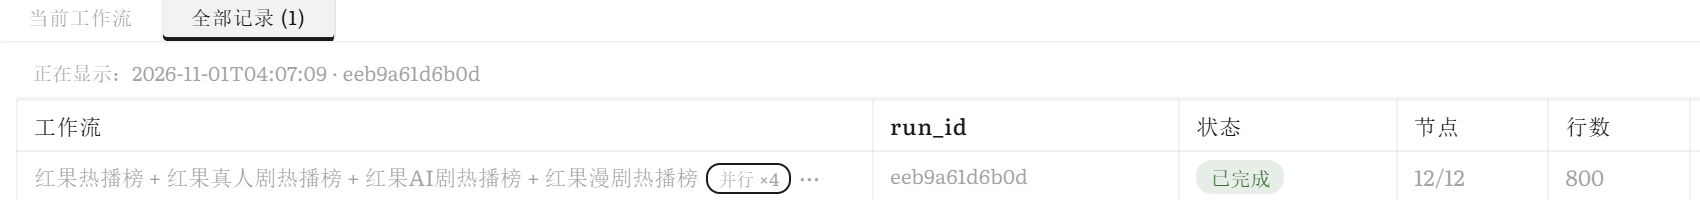
\includegraphics[width=0.96\textwidth]{runs.png}
\caption{运行记录的一行：状态、节点数、行数、耗时与操作}
\label{fig:runs}
\end{figure}

导出产物面板集中显示所有落盘文件，按运行清理，也可以一次清空，下载、删除、复制路径都在每一行上。
运行库会随时间变大，运行记录可以按条删除，导出产物可以按运行清理，删一条运行不动别的运行的行。

数据目录不在版本库里，只有工作流文件例外，所以除了远端仓库还需要一个还原点。备份工具生成一份代码包与一份数据归档，
覆盖系统数据与每个账号自己的库与工作流，默认不含 Cookie。

“\texttt{工作流文件}”面板能导出项目包，包里是工作流、被引用的数据集与可复用模板，换一台机器导入以后接着用，不用重新挂数据。
单独导入一份工作流文件就只是加一份画布。

\begin{figure}[H]\centering
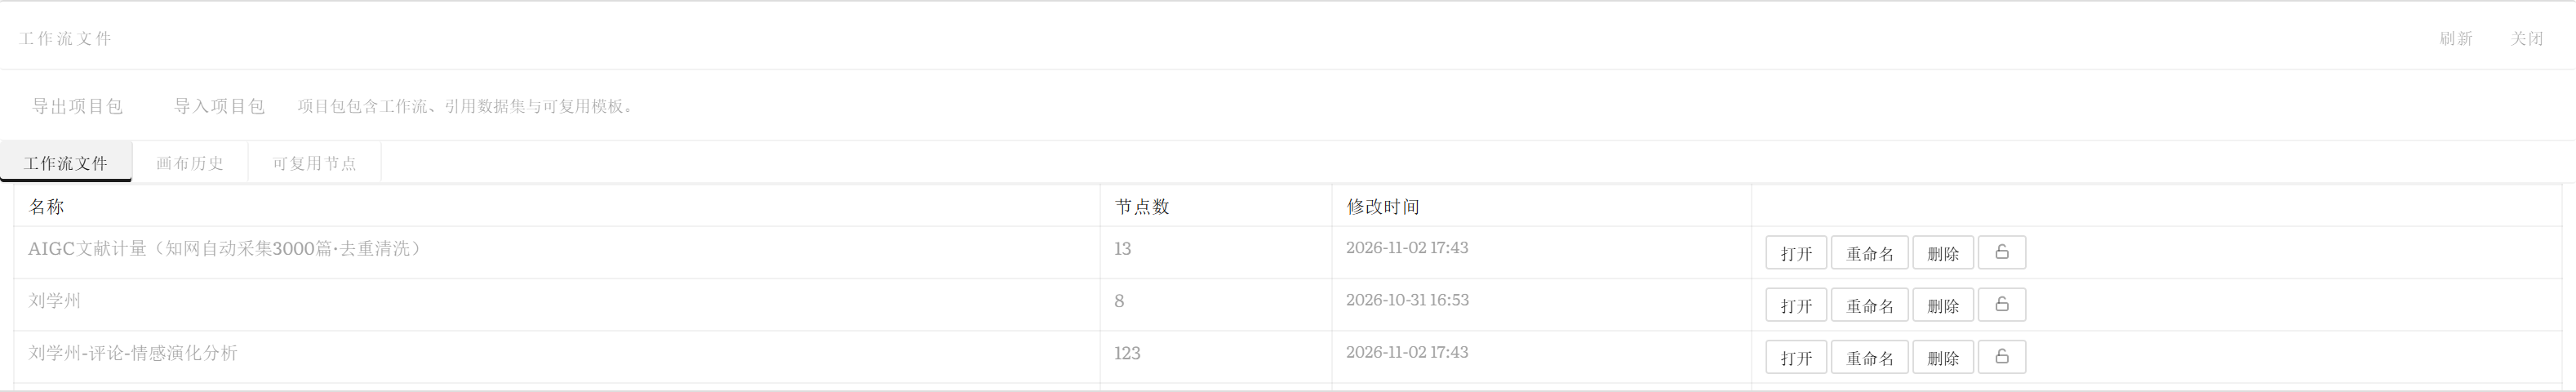
\includegraphics[width=0.92\textwidth]{workflows.png}
\caption{工作流文件：打开、重命名、导入导出、打包成项目}
\label{fig:workflows}
\end{figure}

\section{定时任务}

定时任务由应用内的一只时钟驱动，跟着服务一起启动。到点执行一张已存画布，可以按天、按周、按间隔，也可以写五段 cron；
每个任务可以指定自己的时区，留空按服务器本地时间。面板显示服务器时间、时钟是否在跑、每个任务的下次运行与最近一次结果。

\begin{figure}[H]\centering

\includegraphics[width=0.98\textwidth]{schedules.png}
\caption{定时任务：触发句子、下次运行、启用与立即执行}
\label{fig:schedules}
\end{figure}

含模型节点的画布不能定时。选择画布时就标明不能定时并写出原因，不会等到半夜才失败，因为半夜没人看着花 token 不是好事。

服务停机期间错过的点只记一条已错过，不会在开机时补跑一批。到点的任务与手动执行走同一条启动路径，服务忙就排队；
启动失败写进这个任务自己的历史，不写进运行控制台。下次时间、上次结果、任务句子与能不能跑，全由服务端算好送来，面板不自己猜。

\section{账号与云端}

一个人本机用不需要账号。放到服务器上给多人用就要开云端模式：它会关掉本地模型界面、强制无头抓取、拒绝浏览器生成登录，
并且强制账号登录。已经部署好的那份在 \texttt{http://47.116.114.77/crawler}，打开就能看见登录页；自己开一份也可以，
只要在启动前设好管理员密码与会话密钥，否则按名字拒绝启动。密码用 scrypt 哈希，会话在服务端，带 CSRF 与失败锁定。

\begin{figure}[H]\centering
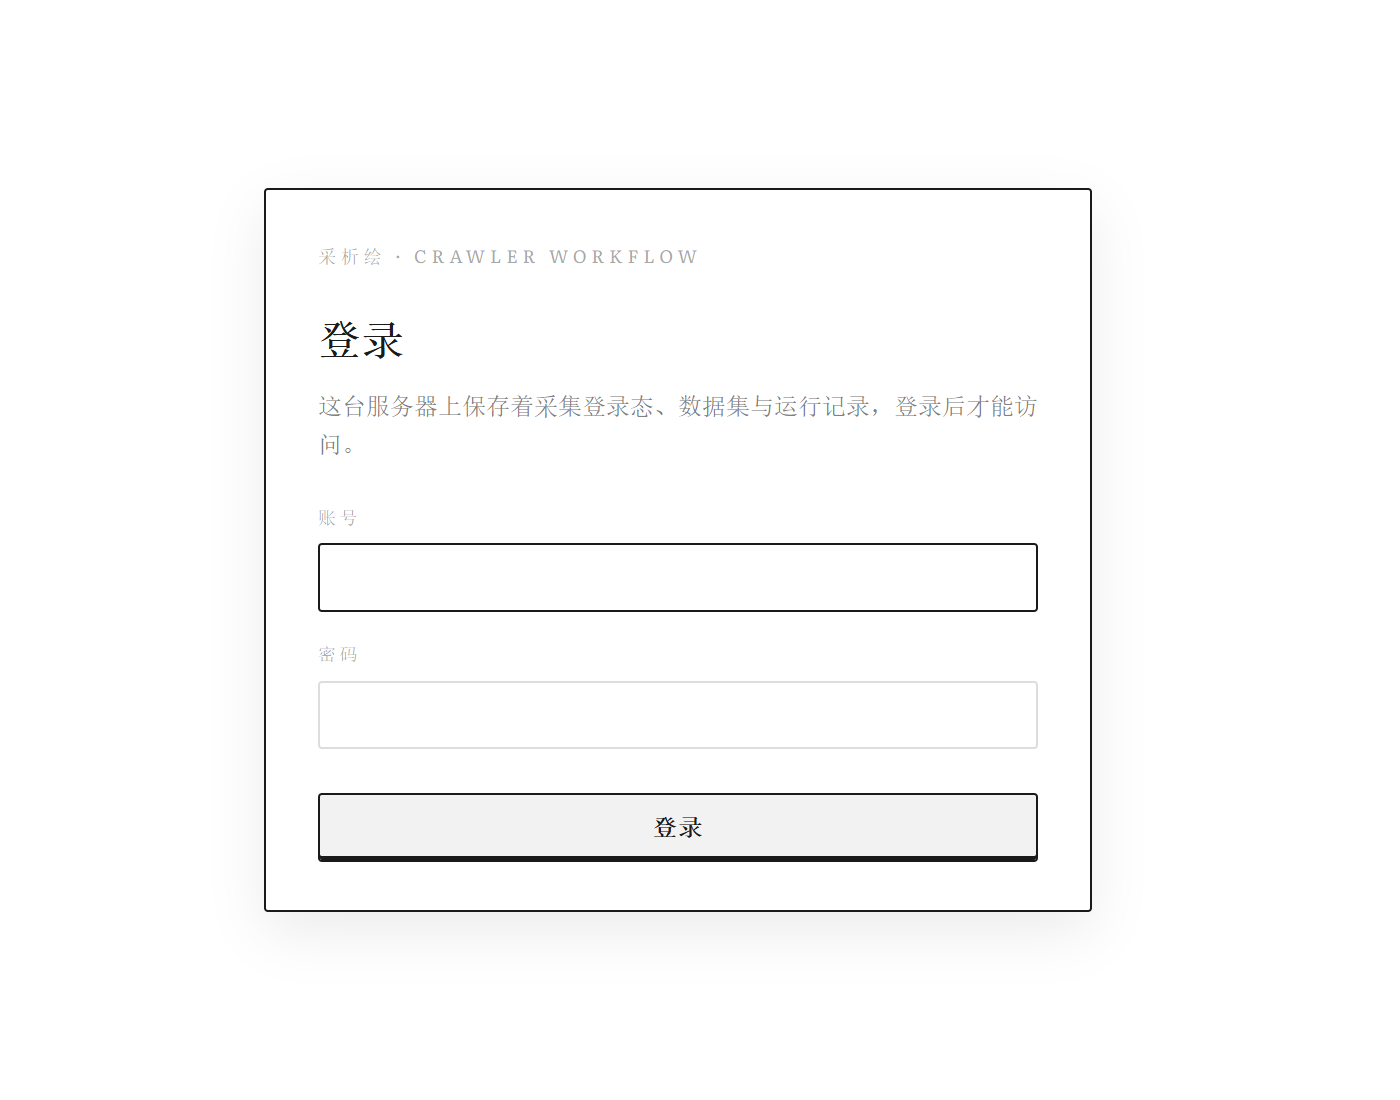
\includegraphics[width=0.5\textwidth]{login.png}
\caption{云端登录页：一条地址，两个输入框}
\label{fig:login}
\end{figure}

密码错一次就是一句话，不会告诉你账号存不存在，也不会告诉你是不是被锁了。连续错到上限会被锁一段时间，这段时间换一个浏览器也没用。
管理员刚开出来的账号带一个临时密码，第一次登录会要求改掉，这一屏不能关；改完以后顶栏右侧出现账号名与退出登录，画布才恢复正常。

\begin{figure}[H]\centering
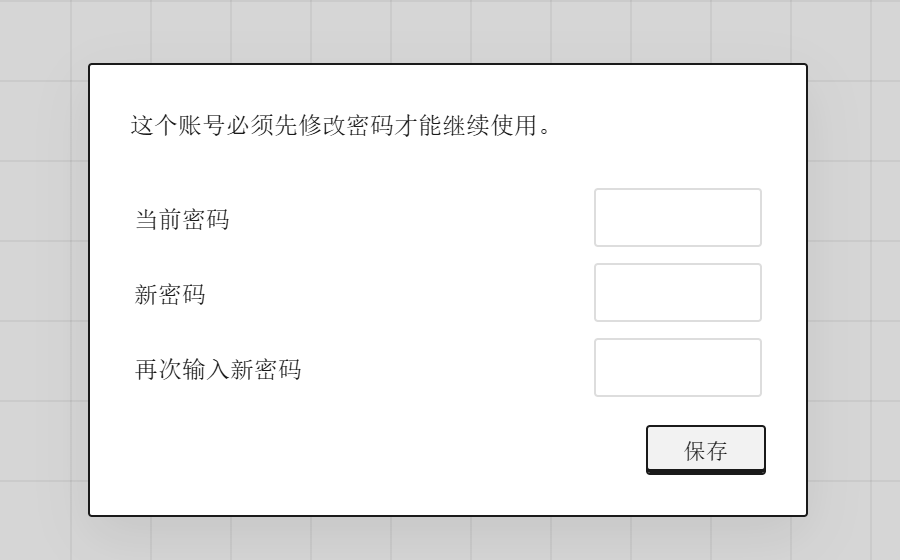
\includegraphics[width=0.44\textwidth]{force-password.png}
\caption{首次登录的强制改密：当前、新、确认}
\label{fig:force-password}
\end{figure}

管理员点顶栏的账号名打开账号管理：上面三个输入框建号，下面一行一个人，能重置密码、强制下线，普通用户还能禁用与删除。
状态列写启用、待改密、已禁用；最近操作是审计，谁在什么时候登录、改密、建号、删号，一条条记着，时间按你所在时区显示。
删除是把这个人整棵数据目录移进回收站，不会当场抹掉；强制下线只踢掉当前会话。

\begin{figure}[H]\centering
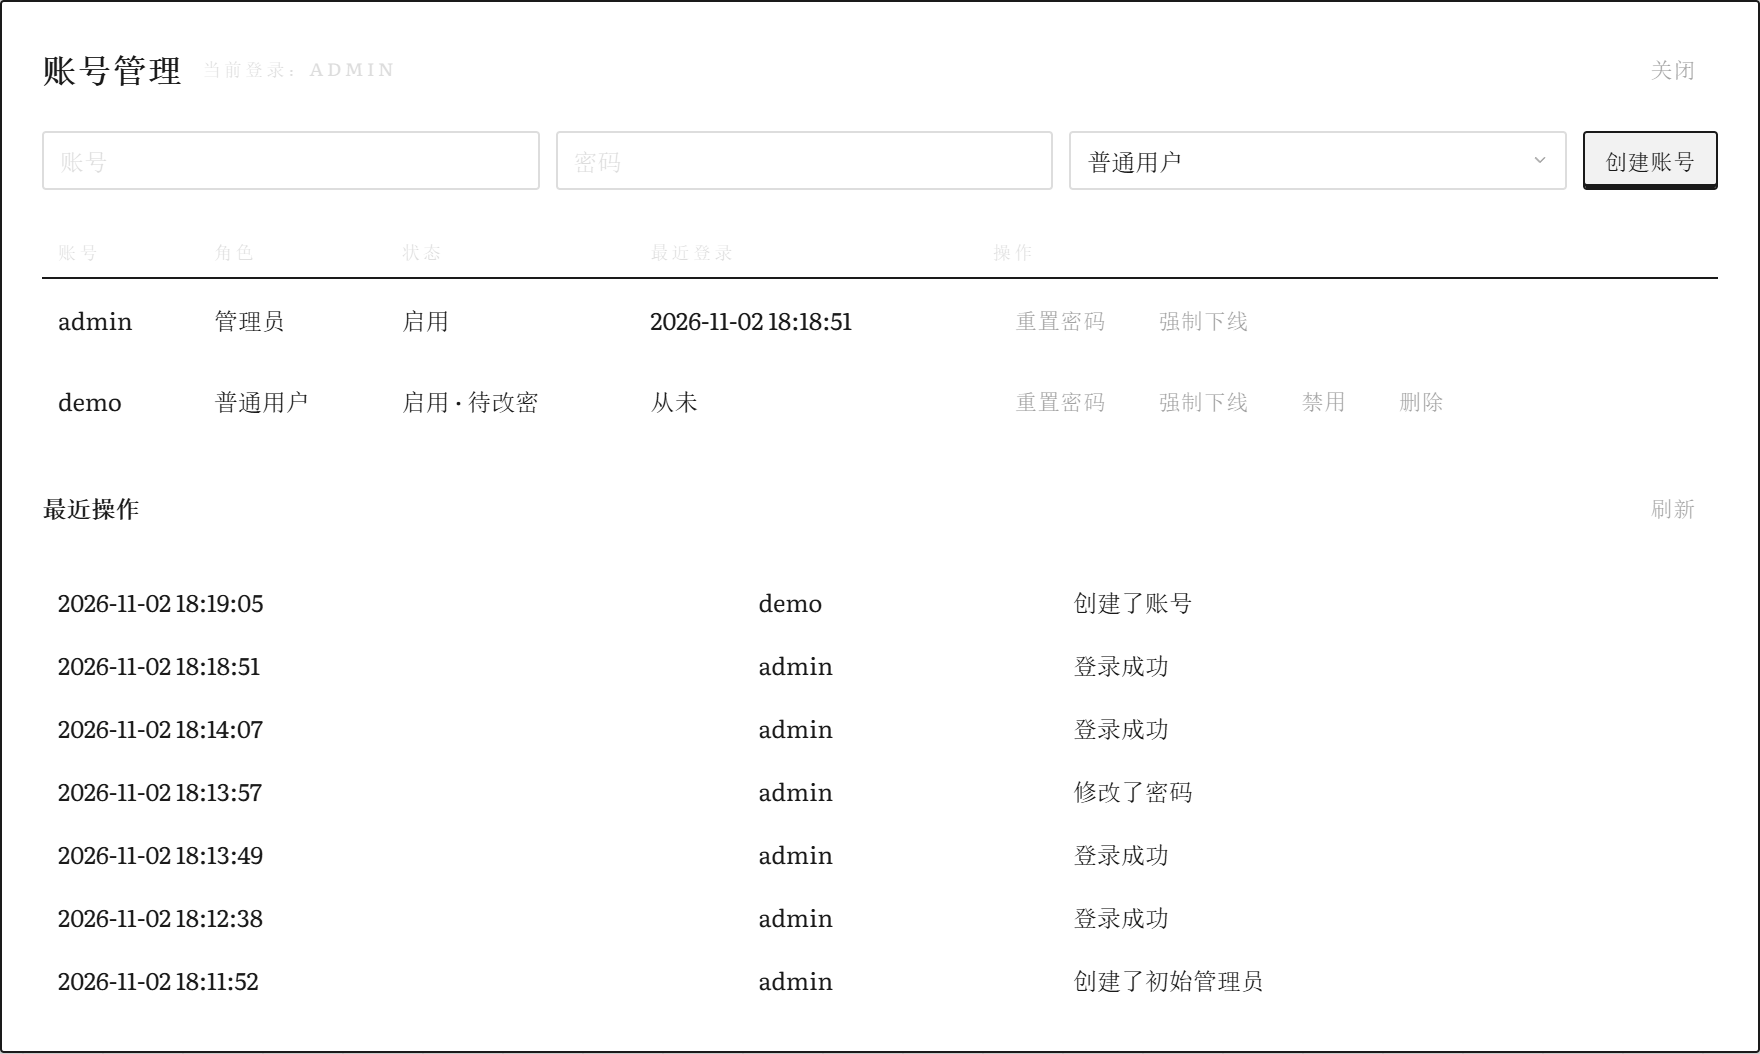
\includegraphics[width=0.94\textwidth]{accounts.png}
\caption{账号管理：角色、状态、最近登录与操作}
\label{fig:accounts}
\end{figure}

每个账号一棵目录树，工作流、数据集、运行记录、登录状态、导出全在里面，运行也互不可见：状态、停止、进程、统计只答自己那一次。
旧版单账号的数据根可以迁到管理员名下，工具默认只演练，确认以后才动手，迁移前先备份，原目录改名保留。

没开账号时把监听地址改成非本机，等于把已保存的登录状态与数据集开放给整个局域网，程序会拒绝启动。这不是多余的限制。

\section{外观、词库与设置}

中英两套文案，切换即时生效，只影响显示，不改数据。主题有自动、浅色、深色三档，自动跟随系统，图表配色一起换。
圆角有一个统一滑杆，改完全界面一起变。

\begin{figure}[H]\centering
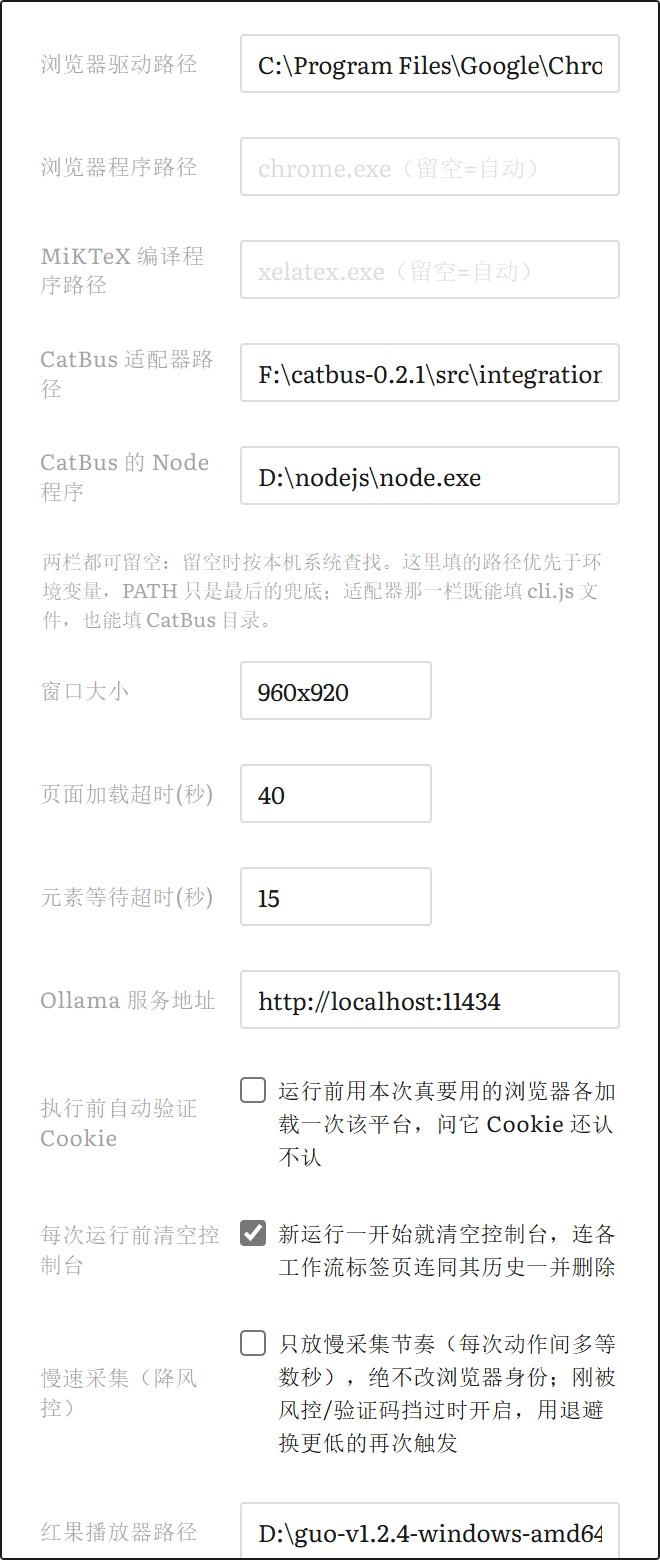
\includegraphics[width=0.5\textwidth]{settings-menu.png}
\caption{设置菜单：驱动路径、浏览器、超时、Cookie 预检、编译程序都在这里}
\label{fig:settings}
\end{figure}

设置面板里能改 Chrome 驱动与浏览器路径、窗口尺寸、页面与元素超时、慢速采集、Cookie 预检开关、同平台排队与错峰，
也能指定编译程序路径与模型服务地址。这些写进配置文件，下次运行直接生效，不用改代码重启。

“\texttt{词库}”面板管停用词与领域词。停用词在关键词、主题、词云与机器学习里都会过滤，领域词写进分词词典，
改动从下一次运行开始生效。

\begin{figure}[H]\centering
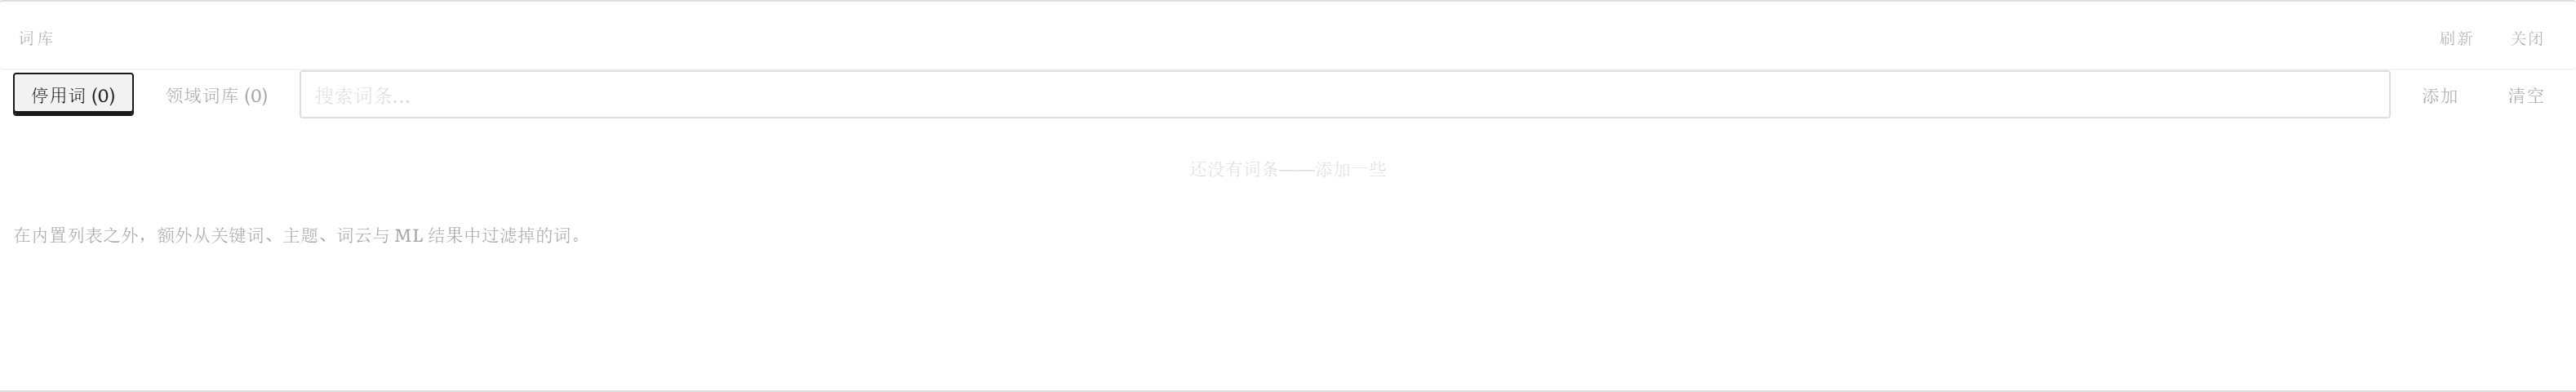
\includegraphics[width=0.43\textwidth]{lexicon.png}
\caption{词库：停用词与领域词}
\label{fig:lexicon}
\end{figure}

深色主题是同一套令牌的另一组取值，图表、节点、面板一起换，导出的 PNG 也跟着换。晚上看画布舒服一些，打印前记得换回浅色。

\begin{figure}[H]\centering
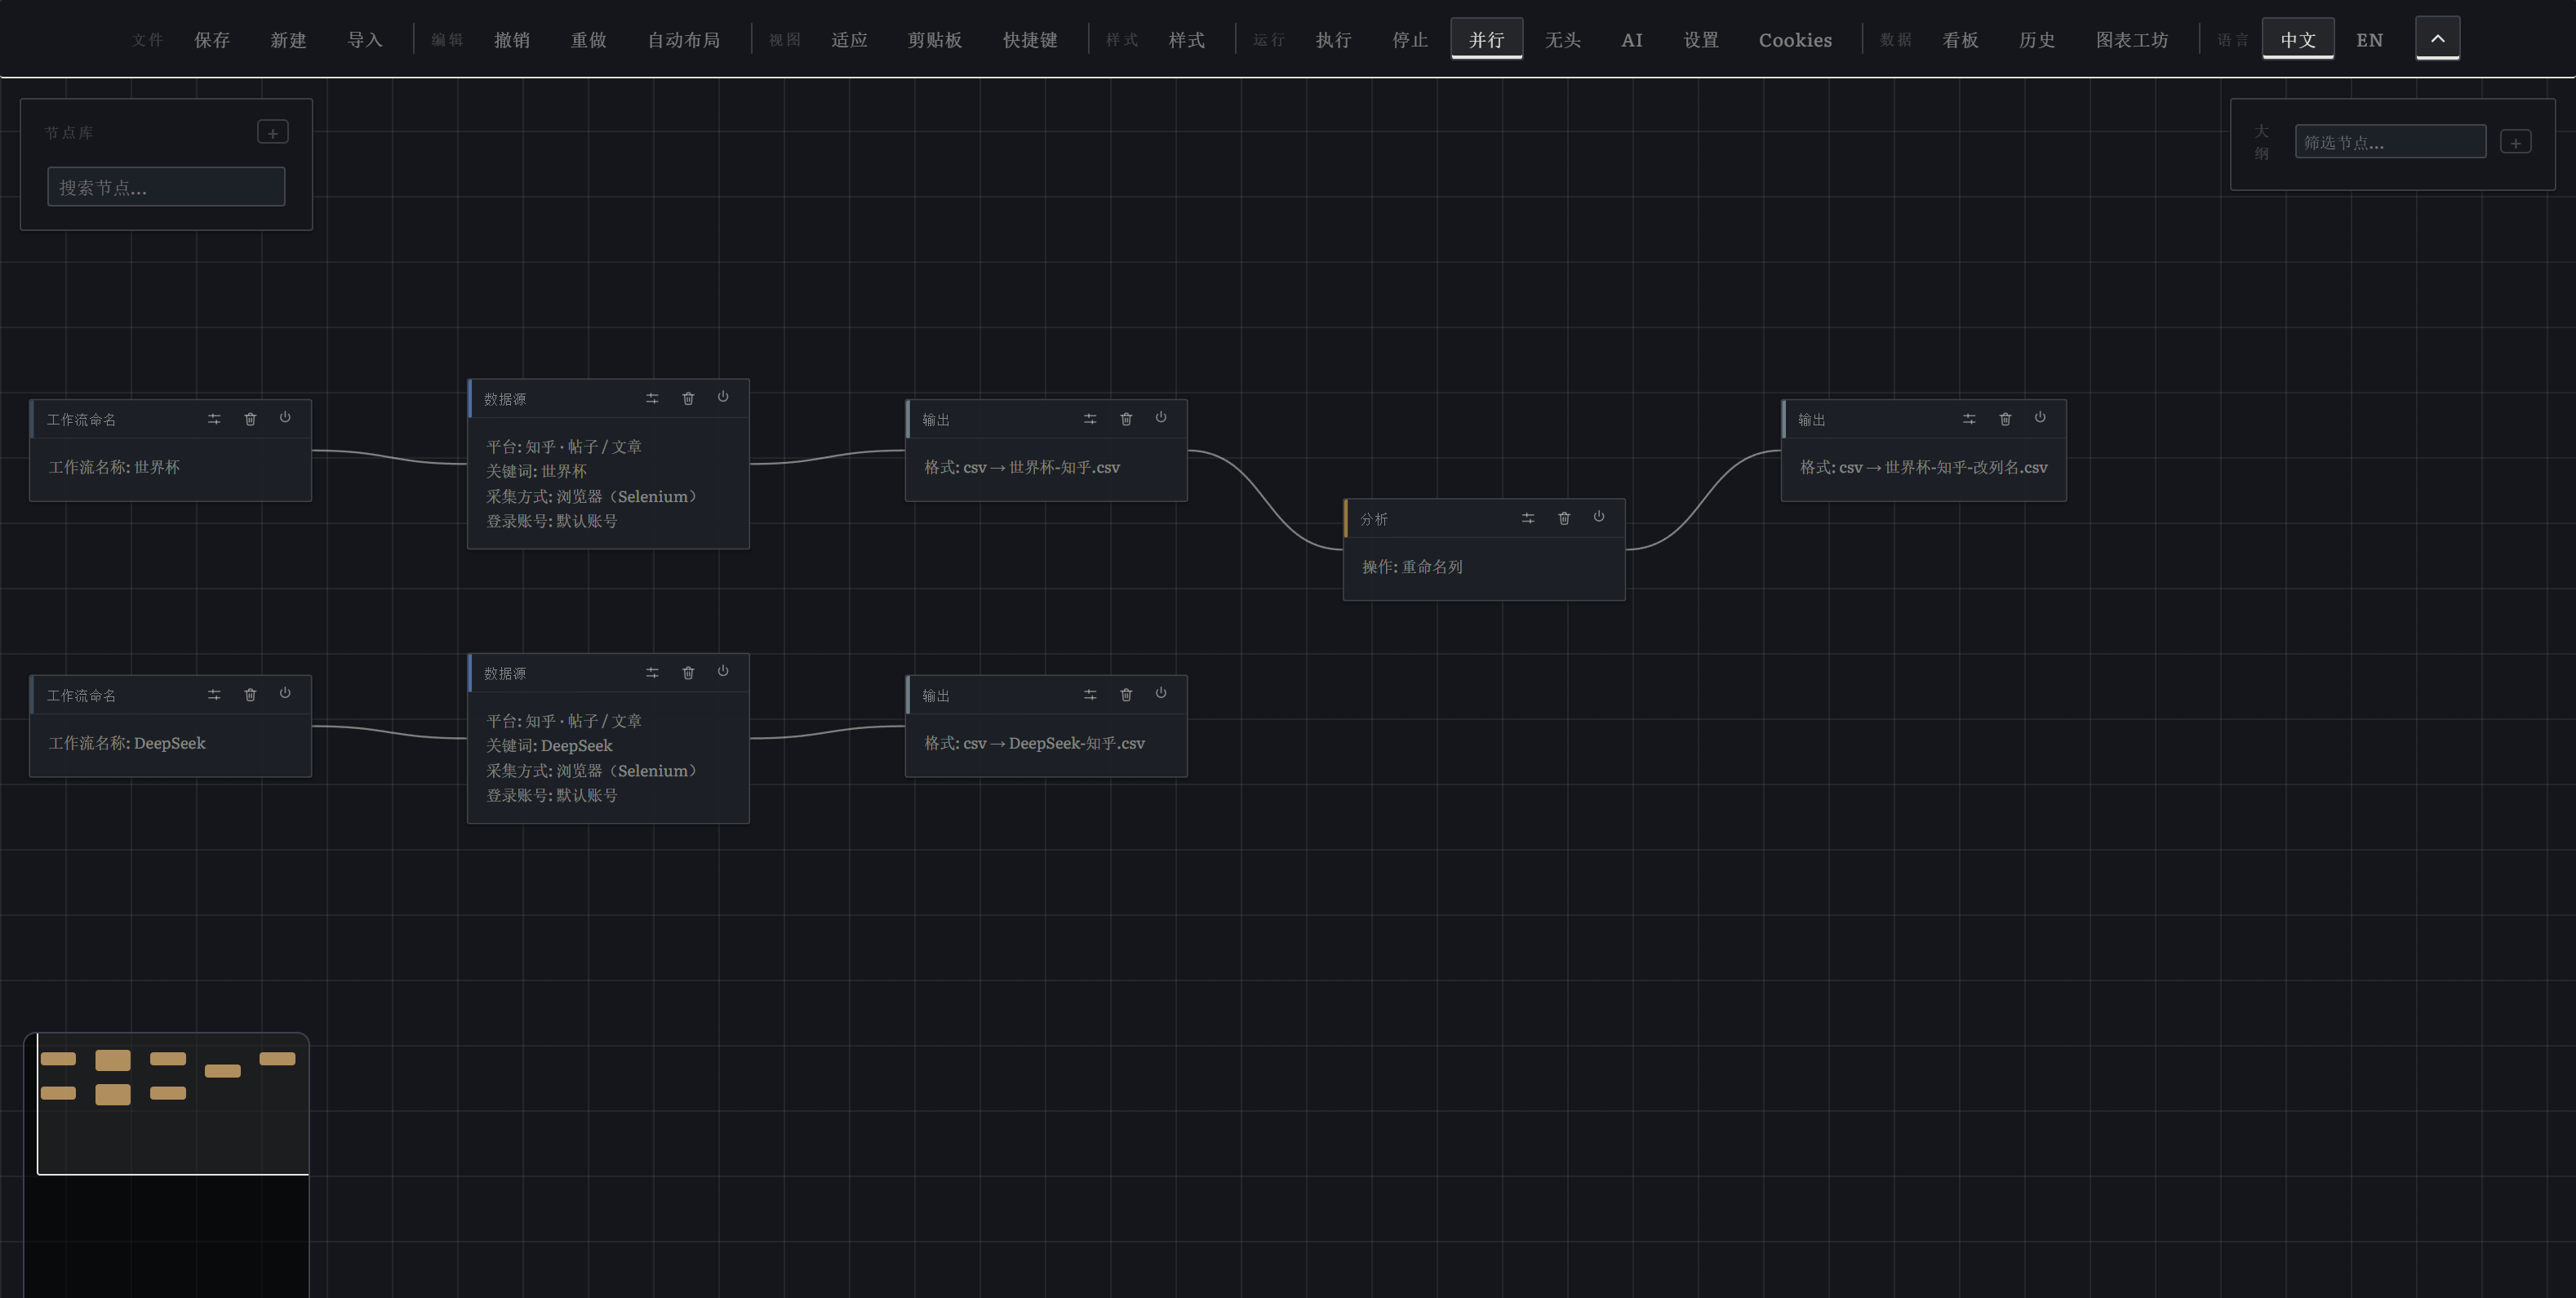
\includegraphics[width=0.96\textwidth]{dark.png}
\caption{深色主题下的画布}
\label{fig:dark}
\end{figure}

\section{打包给别人}

不装 Python 的人用桌面版。它把后端与前端打成一个目录，双击启动本地服务并打开浏览器；数据默认放在用户目录，
exe 旁边放一个空文件就切便携模式，安装包是可选的。微调模型不放应用包里，单独发一个模型包，解压到同级目录自动登记；
不放也能用，相关节点降级并在控制台写明实际用了哪种模式。打包只针对 Windows，Linux 与 macOS 用源码跑，装好 Chrome 与中文字体即可。

\section{被拒绝的时候看哪里}

这个软件遇到不确定的事一律按名字拒绝，不猜。拒绝的话里通常写了原因与下一步。先看控制台那一行，再看节点设置面板顶部的校验提示。

\begin{table}[H]\centering
\caption{常见拒绝与处理}
\label{tab:refuse}
\small
\begin{tabularx}{\textwidth}{p{4.4cm}X}
\toprule
看到的话 & 通常怎么做 \\
\midrule
找不到驱动，或版本不符 & 在设置里填本机 chromedriver 的路径，版本要和 Chrome 一致 \\
登录墙，或账号没有登录状态 & 在 Cookies 面板重新存一份，或换一个已保存的账号 \\
缺模型，或模型跑不动 & 确认 Ollama 在跑、模型名对得上，或换一种分析模式 \\
缺列，或列名不对 & 打开上游节点的设置，看它实际输出哪些列 \\
该组合不可用 & 这个平台没有这个功能，换采集内容或换后端 \\
缺 ctex，或缺 FangSong & TeX 发行版补中文支持，Windows 上装完整版 MiKTeX \\
服务已在运行 & 先停掉旧实例，或给新实例一份自己的数据目录 \\
数据集不在库里 & 换机器时把整个 data 目录一起搬过来 \\
\bottomrule
\end{tabularx}
\end{table}

最后两件小事。数据目录不要随手删，工作流只记数据集编号，换个目录就打不开了；Chrome 驱动不要让工具自己去下载，
本机装好一份、指过去，跑起来最稳。
